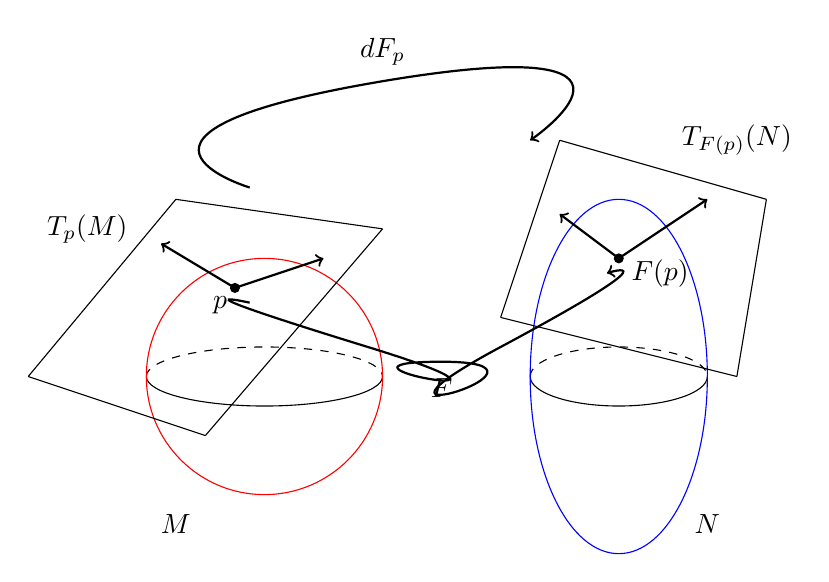
\begin{tikzpicture}[scale=0.75]
  % Esfera
  \draw (-4,0) arc (0:180:2 and -0.5);
  \draw [dashed] (-8,0) arc (180:0:2 and 0.5);
  \draw [red] (-6,0) circle (2);
  \node at (-7.5,-2.5) {$M$};
  \node at (-6.75,1.2) {$p$};
  \node at (-9,2.5) {$T_p(M)$};

  % Rectángulo (Espacio Tangente a Esfera)
  \filldraw (-6.5,1.5) circle (0.075);
  \draw[thick,->] (-6.5,1.5) -- (-5,2);
  \draw[thick,->] (-6.5,1.5) -- (-7.75,2.25);
  \draw  (-7.5,3) -- (-4,2.5);
  \draw  (-4,2.5) -- (-7,-1);
  \draw  (-7,-1) -- (-10,0);
  \draw  (-10,0) -- (-7.5,3);

  % Elipsoide
  \draw (1.5,0) arc (0:180:1.5 and -0.5);
  \draw [dashed] (-1.5,0) arc (180:0:1.5 and 0.5);
  \draw [blue] (0,0) ellipse (1.5 and 3);
  \node at (1.5,-2.5) {$N$};
  \node at (0.7,1.75) {$F(p)$};
  \node at (2,4) {$T_{F(p)}(N)$};

  % Rectángulo (Espacio Tangente a Elipsoide)
  \filldraw (0,2) circle (0.075);
  \draw[thick,->] (0,2) -- (1.5,3);
  \draw[thick,->] (0,2) -- (-1,2.75);
  \draw (-2,1) -- (2,0);
  \draw (2,0) -- (2.5,3);
  \draw (2.5,3) -- (-1,4);
  \draw (-1,4) -- (-2,1);

  % Flechas
  \draw[thick, ->] plot [smooth,tension=4] coordinates {(-6.25,1.25) (-4.25,0.5) (-3,0.25) (-2,0.5) (-0.20,1.75)};
  \node at (-3,-0.20) {$F$};
  \draw[thick, ->] plot [smooth,tension=4] coordinates {(-6.25,3.2) (-4,5) (-1.5,4)};
  \node at (-4,5.5) {$dF_p$};

\end{tikzpicture}
